\subsection{Adapter (\textit{o Wrapper})}
\label{adapter}

\textbf{Scopo}: Strutturale \\
\textbf{Raggio d'azione}: Classi, Oggetti

\paragraph{Definizione} Permette di convertire l'interfaccia di una classe in un'altra interfaccia richiesta dal client.Consente a classi diverse di cooperare quando ciò non sarebbe possibile a causa di interfacce incompatibili.

\paragraph{Motivazione} A volte una classe preesistente, progettata per essere riutilizzata, non può essere riusata perché incompatibile con l'interfaccia richiesta dall'applicazione. Nell’esempio, la classe XXXTriangle non può essere riusata dove ci si aspetta l’interfaccia Figure2D perché non è compatibile con essa.

\begin{multicols}{2}
\begin{figure}[H]
    \centering
    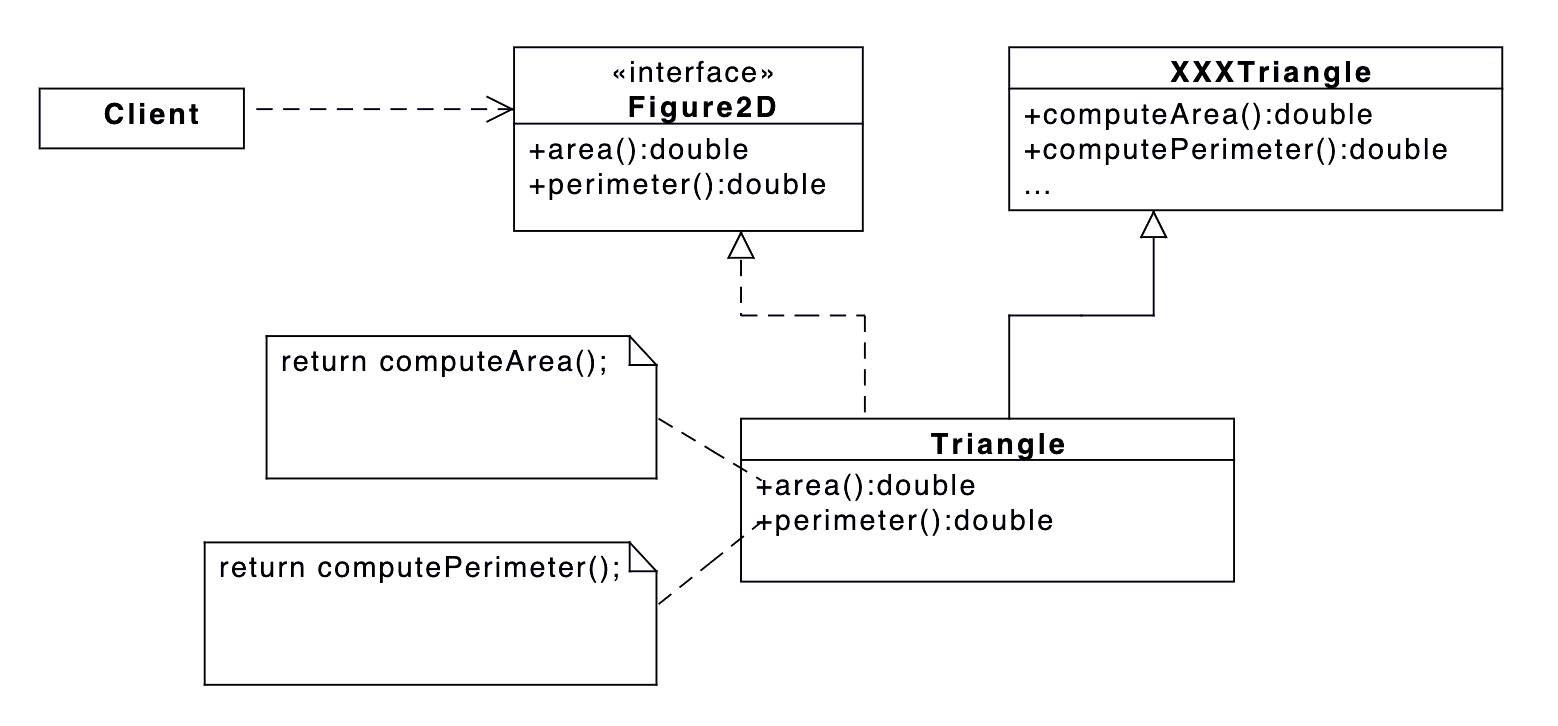
\includegraphics[width=1\linewidth]{assets/pattern/adapter/adapter-esempio-class.png}
    \caption{Esempio di Class Adapter}
\end{figure}
\columnbreak
\begin{figure}[H]
    \centering
    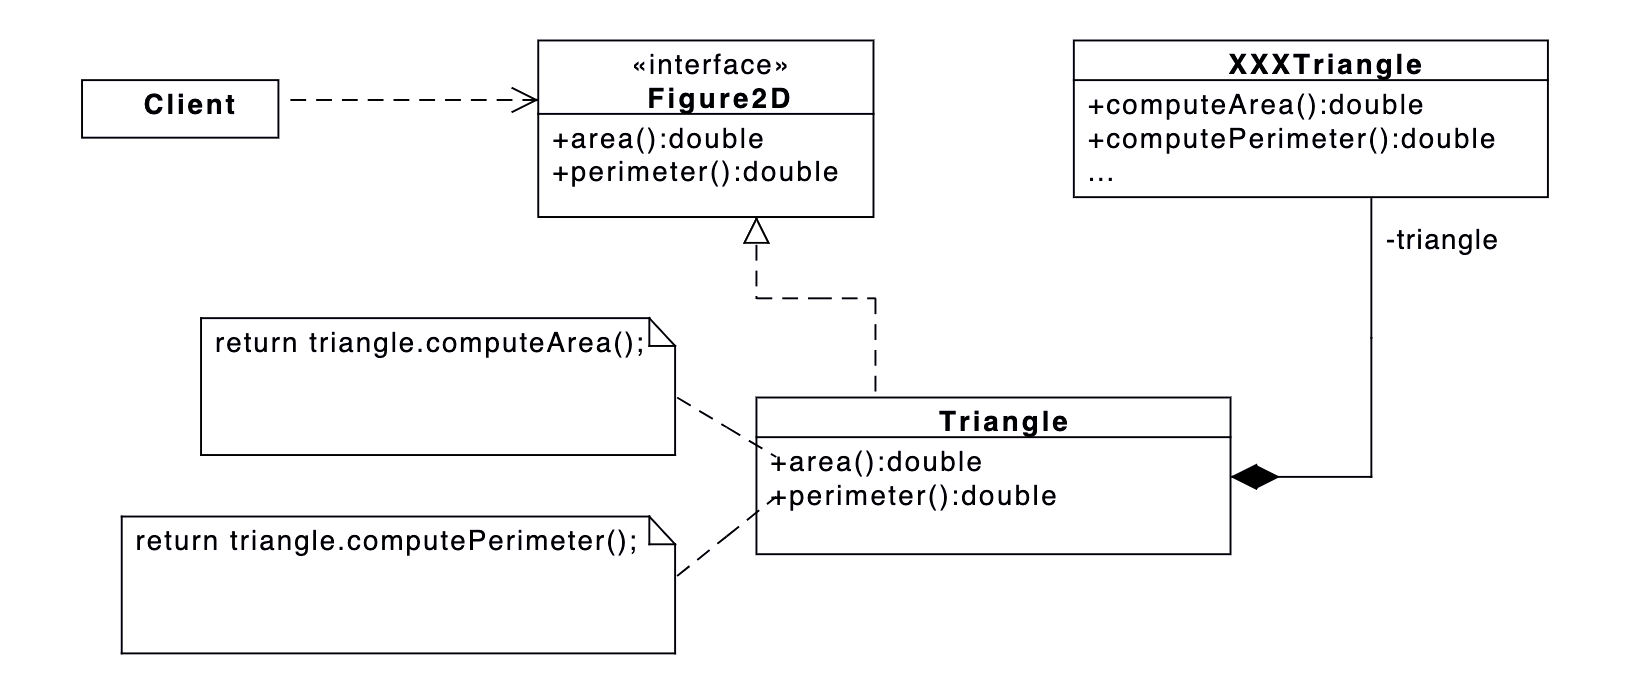
\includegraphics[width=1\linewidth]{assets/pattern/adapter/adapter-esempio-object.png}
    \caption{Esempio di Object Adapter}
\end{figure}
\end{multicols}

Pensare di modificare XXXTriangle per renderla conforme a Figure2D non è una buona soluzione (si legherebbe al contesto specifico e il codice sorgente potrebbe non essere disponibile).

Si introduce una classe Triangle che sia al contempo erede di entrabe XXXTriangle e Figure2D. L'implementazione dei metodi di Figure2D sfrutta quelli di XXXTriangle.

È possibile introdurre la classe Triangle anche di modo che faccia riferimento ad un oggetto (istanza di XXXTriangle) e vada ad implementare l'interfaccia Figure2D delegando l'esecuzione all'oggetto incapsulato.

\begin{figure}[H]
    \centering
    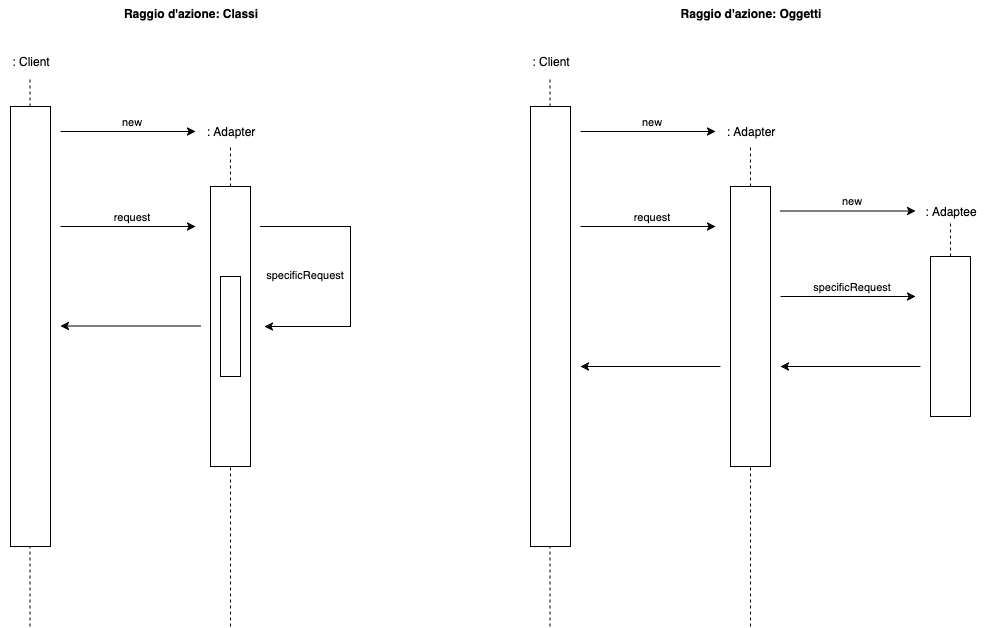
\includegraphics[width=0.75\linewidth]{assets/pattern/adapter/adapter-sequence.drawio.png}
    \caption{Sequence diagram raggio d'azione}
\end{figure}

\paragraph{Applicabilità} È consigliabile utilizzare il pattern Adapter quando:
\begin{itemize}
    \item Si vuole utilizzare una classe esistente e la sua interfaccia non è compatibile con quella che serve;
    \item Si vuole creare una classe riusabile che coopera con classi non correlate o non conosciute;
    \item Si vogliono usare varie sottoclassi esistenti, ma non sarebbe pratico adattare le loro interfacce tramite ereditarietà (solo per object);
\end{itemize}

\paragraph{Struttura} Il pattern è composto dai seguenti partecipanti:
\begin{itemize}
    \item \textbf{Target} (Figure2D): definisce l'interfaccia specifica del dominio utilizzata dal client
    \item \textbf{Client}: collabora con oggetti compatibili con l'intefaccia Target
    \item \textbf{Adaptee} (XXXTriangle): individua un'interfaccia che deve essere adattata.
    \item \textbf{Adapter} (Triangle): adatta l'interfaccia Adaptee al'interfaccia Target
\end{itemize}

I client invocano le operazioni su un'istanza di Adapter, il quale invoca operazioni di Adaptee per soddisfare la richiesta

\begin{figure}[H]
    \centering
    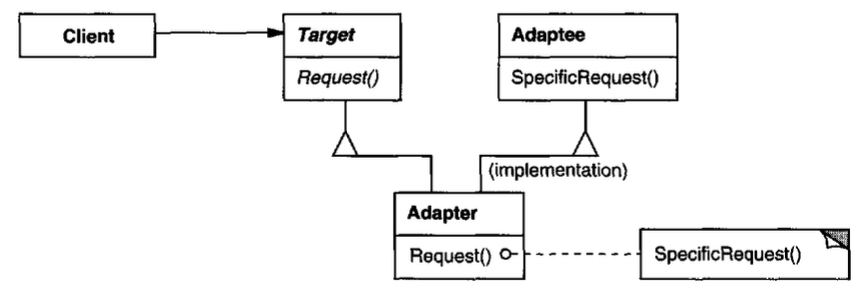
\includegraphics[width=0.75\linewidth]{assets/pattern/adapter/adapter-struttura-class.png}
    \caption{Class Diagram di Adapter (Class)}
\end{figure}

\begin{figure}[H]
    \centering
    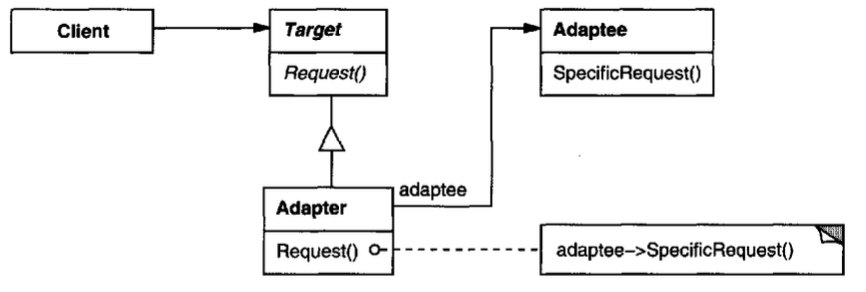
\includegraphics[width=0.75\linewidth]{assets/pattern/adapter/adapter-struttura-object.png}
    \caption{Class Diagram di Adapter (Object)}
\end{figure}

\paragraph{Conseguenze} Il pattern Builder consente quindi di:
\begin{itemize}
    \item Scegliere lo spettro di operazioni da supportare (o wrappare);
    \item Supportare i \textbf{pluggable adapter}: classi che supportano l'adattamento di interfaccia
    \item Usare i \textbf{two-way adapters}: permettono all'Adapter di supportare operazioni dell'Adaptee e viceversa.
\end{itemize}

\textbf{Class Adapter}
\begin{itemize}
    \item Adatta l'interfaccia Adaptee all'interfaccia Target basandosi su una classe concreta.
    \item Non può essere utilizzata se Adaptee è astratta oppure è un'interfaccia.
    \item Consente ad Adapter di sovrascrivere parte del comportamento di Adaptee essendo una sua sottoclasse
    \item Non occorrono ulteriori indirezioni per raggiungere l'oggetto adattato
\end{itemize}

\textbf{Object Adapter}
\begin{itemize}
    \item Permette ad un singolo Adapter di operare con Adaptee e le sue sottoclassi, se esistono. Può in tal caso aggiungere funzionalità a tutti gli Adaptee
    \item Rende difficile sovrascrivere il comportamento di Adaptee non essendo una sua sottoclasse
    \item Aggiunge un livello di indirezione per raggiungere l'oggetto adattato.
\end{itemize}

\newpage